\chapter{Verification and validation}
\label{ch:verify}

\section{Approach}
Verification asks whether the equations were solved correctly; validation asks whether they are the right equations. The checks here address the first question for every component and the second for the half-space model, by comparing it with the finite element block. A simulator can be wrong in ways that look reasonable: a plausible picture with a wrong number. The checks here therefore compare the code with something independent: a closed-form result, a limiting case where the answer is known, an invariant that must hold for \emph{any} input, or a second implementation of the same physics. Where an exact answer is not available, a numerical experiment (mesh refinement, growing the body) shows the trend toward one.


The counts in the table below were recorded during development, when each check was a scripted test. The test files were removed from the repository at the owner's request, so these counts are a record of that work and are not re-run by the build. The two sections that follow were re-run while preparing this report.

\begin{table}[H]\centering\small
\caption{Checks recorded during development, by component.}\label{tab:checks}
\begin{tabular}{@{}p{3.1cm}p{1.9cm}p{9.8cm}@{}}\toprule
Component & Checks & What was verified\\\midrule
\texttt{physics.js} & 54 & invariants and ordering of the principal stresses for 4000 random tensors over 12 decades of stress; hydrostatic, uniaxial, pure-shear and double-root cases; Boussinesq and Cerruti satisfy $\nabla\!\cdot\tens\sigma=\mathbf0$ at random points for several $\nu$; the Boussinesq stress equals Hooke's law applied to the gradient of its displacement; $\int\sigma_z\,dA=-P$ on four depths; the surface is stress-free outside the load; far-field decay; singular points stay finite\\
\texttt{server.py} & 40 & eigen-decomposition against numpy; $|\mathbf t|^2=\sigma_{nn}^2+\tau^2$; the section is linear in load, obeys the triangle inequality for superposed loads, is symmetric, is zero for zero load, is hydrostatic for full coverage, has the right cylinder and sphere masks; and the browser physics agrees with the server for four load orientations to $2\times10^{-4}$\\
Simulators & 110 & each closed form (Chapters~\ref{ch:stress} and~\ref{ch:sims}) plus limits, listed below\\
Simulators, random & 22\,500 & 2500 random or extreme inputs for each of nine simulators: no exception, no NaN, and the only infinite values are safety factors with no load\\
FEM & 43 & patch test, closed forms, equilibrium, full-pressure block, growing the block toward the half-space, 116 extreme inputs\\
3D tab & 94 & every shape, material, load type and map with painted loads, no non-finite output, no console error\\\bottomrule
\end{tabular}
\end{table}

\section{Limiting cases of the simulators}
\begin{center}\small
\begin{tabular}{@{}p{2.7cm}p{12.3cm}@{}}\toprule
Simulator & Limits checked\\\midrule
Mohr & uniaxial $(\sigma_1=\sigma,\ \tau_{\max}=\sigma/2)$; hydrostatic $(\tau_{\max}=0,\ \sigma_{vM}=0)$; pure shear $(\sigma_{vM}=\sqrt3\tau)$; 400 random states: the transformation law, $\sigma_{x'}+\sigma_{y'}$ invariant, $\sigma_1+\sigma_2+\sigma_3=I_1$, $\sigma_1\sigma_2\sigma_3=I_3$, $\sigma_{vM}^2=I_1^2-3I_2$\\
Beam & simply supported central load ($M=PL/4,\ \delta=PL^3/48EI$), UDL ($wL^2/8,\ 5wL^4/384EI$), cantilever tip load, UDL and end moment, moment at a support, equilibrium of reactions, load at a support, $a>L$ clamp, zero load; Timoshenko shear term $=PL/4k_sGA$, tends to Euler--Bernoulli for slender beams and dominates for stubby ones; $1.5V/A$, $4V/3A$ and $2V/A$ (thin tube) shear stresses; circle and tube properties\\
Shaft & $16T/\pi D^3$, $TL/GJ$, hollow $J$, $\tau_{\min}=\tau_{\max}d/D$, thin-wall $T/2\pi r^2t$, zero torque, solid limit, linearity, $\phi\propto L/D^4$\\
Axial & elongation $=\sum NL/EA$, fixed--fixed net elongation zero, thermal $-E\alpha\Delta T$ (fixed) and $\alpha\Delta T\,L$ (free)\\
Pressure vessel & Lam\'e cylinder and sphere inner and outer hoop stress, external pressure, equal pressures (hydrostatic), zero pressure, thin-wall limit, inflation $u=\frac{a}{E}[\sigma_\theta-\nu(\sigma_r+\sigma_z)]$, von Mises from the Lam\'e stresses\\
Thermal & $-E\alpha\Delta T$, $/(1-\nu)$, $/(1-2\nu)$; half restraint gives half the stress; $\Delta T=0$; cooling gives tension; $\Delta T$ to yield\\
Failure & uniaxial tension and compression: all four theories agree; pure shear: Tresca $\sigma_y/2\tau$, von Mises $\sigma_y/\sqrt3\tau$, Rankine $\sigma_y/\tau$, St Venant $\sigma_y/[\tau(1+\nu)]$; hydrostatic: Tresca and von Mises never fail; equal biaxial tension; unsorted input; doubling the stresses halves each factor; Tresca $\ge$ von Mises $\ge\tfrac{\sqrt3}{2}$Tresca\\
Energy & all four members with and without shear: Castigliano equals closed form, $U=\tfrac12P\delta$, reciprocity $\delta_{ab}=\delta_{ba}$\\
Buckling & $\pi^2EI/(KL)^2$ for the four end conditions, weak-axis choice, $1/L^2$ scaling, transition slenderness $\pi\sqrt{E/\sigma_y}$, short columns flagged and capped at yield, zero load, slender column\\\bottomrule
\end{tabular}
\end{center}


\section{Default cases against closed forms (re-run)}
\label{sec:defaults}
Each simulator was opened in the running application with its default inputs, and the displayed result was compared with an independent evaluation of the closed-form expression (a separate script using NumPy, with $E=200$~GPa and $\nu=0.3$). Table~\ref{tab:defaults} lists the comparison. Every quantity agrees to the printed precision.

\begin{table}[H]\centering\small
\caption{Application output for the default inputs of each simulator against an independent closed-form evaluation.}\label{tab:defaults}
\begin{tabular}{@{}llrrr@{}}\toprule
Simulator & Quantity & Application & Closed form & Unit\\\midrule
Mohr, $(80,-20,0,\tau_{xy}=-39)$ & $\sigma_1$ & 93.41 & 93.41 & MPa\\
 & $\tau_{\max}$ & 63.41 & 63.41 & MPa\\
 & $\tau_{x'y'}$ at $38^\circ$ & $-57.95$ & $-57.95$ & MPa\\
 & von Mises $\sigma_{eq}$ & 113.9 & 113.9 & MPa\\
Beam, $80\times160$ mm, $P=10$ kN, $L=3$ m & $M_{\max}$ & 7.50 & 7.50 & kN\,m\\
 & $\sigma_{\max}$ & 21.97 & 21.97 & MPa\\
 & $\delta_{\max}$ & 1.03 & 1.03 & mm\\
Shaft, $D=50$ mm, $T=800$ N\,m & $\tau_{\max}$ & 32.59 & 32.59 & MPa\\
 & twist $\varphi$ & 1.17 & 1.17 & deg\\
Axial, three segments & $\sigma_{\max}$ & 87.50 & 87.50 & MPa\\
 & elongation & 0.338 & 0.338 & mm\\
Pressure vessel, $a=200$, $t=12$, $p=10$ MPa & Lam\'e hoop at bore & 171.8 & 171.8 & MPa\\
 & von Mises at bore & 157.5 & 157.5 & MPa\\
Thermal, $\Delta T=60$ K, fully restrained & $\sigma=-E\alpha\Delta T$ & $-144.0$ & $-144.0$ & MPa\\
Failure, $(150,60,0)$ & von Mises & 130.8 & 130.8 & MPa\\
Energy, cantilever, $P=2$ kN & $U$ & 26.53 & 26.53 & J\\
Buckling, $30\times50$ mm, $L=2$ m & $P_{cr}$ & 55.52 & 55.52 & kN\\
 & slenderness $\lambda$ & 230.9 & 230.9 & ---\\\bottomrule
\end{tabular}
\end{table}

\section{Convergence of the finite element solver (re-run)}
\label{sec:convergence}
Figure~\ref{fig:conv} shows three mesh studies run through the solver's HTTP interface.

\begin{figure}[t]
\centering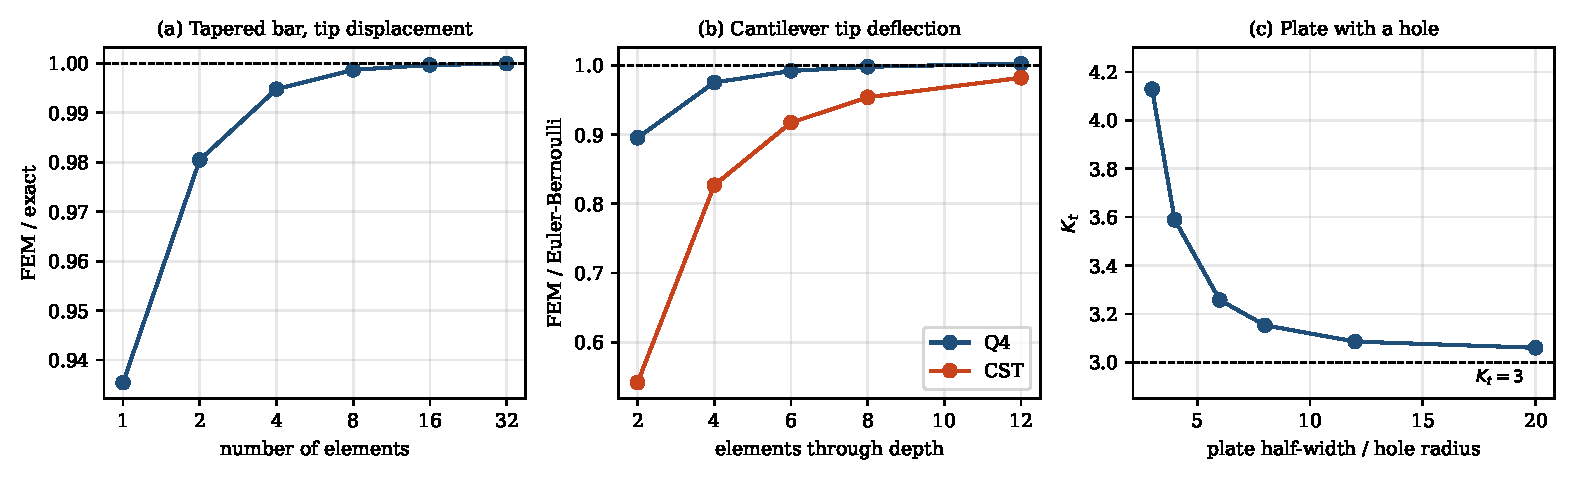
\includegraphics[width=\linewidth]{../figures/fem_convergence.pdf}
\caption{Convergence of the finite element solver. (a) Tip displacement of the tapered bar divided by the exact value, against the number of elements; the error falls from $6.5\%$ with one element to $0.01\%$ with thirty-two. (b) Tip deflection of a plane-stress cantilever divided by Euler--Bernoulli theory, for the four-node element (Q4) and the constant strain triangle (CST); CST is much stiffer on coarse meshes. (c) Stress concentration factor of a plate with a hole, against the ratio of the plate half-width to the hole radius; the dashed line is the infinite-plate value $K_t=3$.}\label{fig:conv}
\end{figure}

\begin{itemize}[nosep]
\item \textbf{Bar} (a): the ratio is $0.935$ with one element and $0.9999$ with thirty-two. The error falls roughly by a factor of four per doubling, the rate expected for linear elements.
\item \textbf{Cantilever} (b): Q4 reaches $0.998$ with eight elements through the depth; CST reaches only $0.954$ at the same density. Both underestimate the deflection on coarse meshes (the elements are too stiff in bending), so a structure dominated by bending needs either Q4 or a finer mesh. The Q4 ratio at twelve elements, $1.002$, is slightly above one because Timoshenko shear deformation adds to the Euler--Bernoulli deflection.
\item \textbf{Hole} (c): $K_t$ falls from $4.13$ for a plate only three radii wide to $3.06$ for twenty. The finite width raises the peak, and the result tends to the Kirsch value of $3$ from above, as it should. The mesh limit of the dense solver (about 3600 degrees of freedom) prevents a finer study at the widest ratios.
\end{itemize}

\section{Further checks of the finite element code (recorded)}
\begin{center}\small
\begin{tabular}{@{}p{5.8cm}p{9.2cm}@{}}\toprule
Test & Result\\\midrule
Patch test, CST and Q4, irregular mesh & uniform stress reproduced to $10^{-8}$\\
Uniform bar & exact at any mesh\\
Tapered bar & ratio to exact $0.935\to0.9999$ (1 to 32 elements)\\
Beam, tip load and UDL & nodal deflection exact to $10^{-9}$ with 1 element, $L/h=2$ and $250$\\
Plane-stress cantilever, Q4, $\nu=0\ldots0.499$ & within $1.7\%$ of Timoshenko on a $12$-element depth mesh\\
Coarse slender cantilever ($L/h=40$) & Q4 $0.89$ and CST $0.54$ of theory: shear locking is real, and noted\\
Plate with a hole & $K_t=3.10\ (W/a=12)$, $3.17\ (8)$, $3.60\ (4)$: the finite-width trend toward $3$ (Kirsch~\cite{kirsch}; see also~\cite{peterson})\\
Block, full-face pressure & $\sigma_z=-q$ everywhere, $\sigma_x=\sigma_y=0$, crush $-qH/E$\\
Block, patch load & centre stress $1.26$, $1.06$, $1.03$ times the half-space value for blocks of $2\times3$, $4\times4$, $8\times8$ m; side-face $\sigma_x$ about $0.4\%$ of $q$ against $2.6\%$\\
Reactions & equal the applied load to rounding in all cases and on 116 extreme inputs\\\bottomrule
\end{tabular}
\end{center}

\section{Defects found by the tests, and what was changed}
Each of the following was found by a limiting-case test and then corrected; the original behaviour is stated so that the reason for the code can be understood.
\begin{enumerate}
\item \textbf{Torsion in the energy tab} (\file{sims.js}, \texttt{energy.compute}). The closed-form displacement and the work were $10^6$ too small because the torque was converted twice. The status check had a special case that skipped torsion, which hid the error. Both corrected.
\item \textbf{Short columns} (\texttt{buckling.compute}). Euler's critical stress was reported even above yield (up to $4\times10^4$~MPa) and the safety factor used it. A Johnson parabola now governs when $\lambda<\lambda_c$.
\item \textbf{Principal stresses} (\file{physics.js}, \texttt{principalStresses}; \file{sims.js}, \texttt{eig3}). A fixed threshold on $J_2$ treated small non-hydrostatic stress states as hydrostatic. The threshold is now relative to the stress scale.
\item \textbf{$\nu=0.5$} (\texttt{tangentialTensor} and \file{server.py}). The Lam\'e constant divides by $1-2\nu$: infinite stress in the browser and a division-by-zero error on the server. The value is capped at $0.499$ in that formula.
\item \textbf{Section endpoint}. A resolution below 2 crashed the request and a force direction that was not a unit vector scaled the load. Resolution is clamped (2 to 400) and the direction is normalised. Earlier in the project the section used the wrong axis for cylinders and drew stress outside the body; both were corrected.
\item \textbf{Display}. An infinite safety factor appeared as a dash and now shows $\infty$. Strains above $1\%$ carry a warning.
\item \textbf{Finite plate with a hole} (not a defect but a result): the first Kirsch comparison showed $K_t$ above $3$; the trend with the width ratio explains this.
\end{enumerate}

